\documentclass{article}
\usepackage[margin=1in]{geometry}

\usepackage{graphicx}

\title{Project proposal}
\author{Colby Goettel\and Amanda Beatty}

\begin{document}
\maketitle

\section{Problem description}
% Clear description of problem addressed, benefits etc.

% add use cases
The main problem being addressed is that neither Amanda nor Colby know too much about mechatronics and this project is a great learning platform for learning a variety of ideas and applications.

One major problem that we'll run into as we go about this project is that the teddy bear needs to remain soft and cuddly and not creepy. To solve the soft and cuddly part, we will use light and semi-flexible components in those big, hugging arms. Components like plastics and stiff-ish foam will help to give support to the body while still allowing the bear to be cuddly.

To be non-creepy, we'll make sure Colby's voice isn't used for the bear. Additionally, we're going to work hard on how the light and temperature sensors are installed so that the bear is still aesthetically pleasing. Finally, no camera will be installed because that's creepy from any angle.

One of the biggest issues that will be addressed is power consumption. We are going to work hard on lowering the power requirements, especially because we'll need two batteries: one to drive the board and another to drive the motors. Any corners that can be cut to save power will be pursued.

The overarching system design is shown in Figure~\ref{fig:system}.

\begin{figure}[h!b]
    \centering
    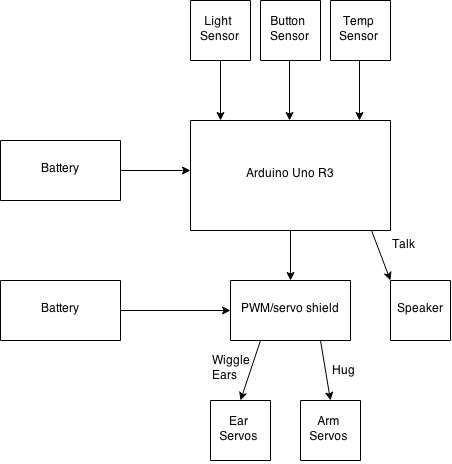
\includegraphics[width=0.6\textwidth]{basic-structure}
    \caption{Basic design of the system.}
    \label{fig:system}
\end{figure}

\subsection{Software modules}
The entirety of this project is going to be written in C. Arduino libraries will be used as much as possible, especially for servo control. Since no SBC will be used, there will not be any Python or other code~--- only C.

\section{Proposed system}
% Clear description of proposed system
\subsection{Brains}
The bear is going to be controlled by an Arduino Uno R3 with a PWM shield attached to the top. This will allow us to drive the four servos (more on that in a minute) from the board. The Arduino and the shield will be attached so they must be stored in the same place. Each needs a separate battery pack to run.

\subsection{Wiggly ears}
Two mini-servos will be installed in the ears to make them wiggle. These will also be driven by the PWM bridge.

\subsubsection{Thermal sensor}
A thermal sensor will be installed in the mouth that will be able to detect if a person is kissing it (quick change in relative temperature). This will trigger the wiggling ears.

\subsection{Big, hugging arms}
The bear will have robotics in the arms that allow it to hug. This will be driven by regular size servos. Hoping that the plastic gear servos can give enough torque for the arms to hug. If not it's another \$40 for metal gear servos (not the end of the world, but that's a lot of tacos).

Still trying to figure out when we want the arms to be actuated. Thinking about installing a button in one of the hands, but that doesn't make much sense. Any ideas? We're going to reserve kissing it (the thermal sensor) for wiggling its ears. That seems the cutest.

\subsection{Light sensor}
A light sensor will be installed in the eye to detect if it's getting dark out. One possible use for this bear is as a child's companion. As such, it would be good to be able to tell the kid that it's getting dark out them and have them head home. It will be necessary to program the system to not constantly say, ``It's getting dark out,'' but rather say it once every 5~minutes (or something). I'd venture to say that this is the least essential system.

\subsection{Sitting position}
Because the bear will default to sitting, we'll have to add additional weight to it's rear to help it stay upright while supporting the weight of the components. This is another reason we'll be using light components.

\subsection{Speaker}
A speaker will be installed (probably on the board for ease) that will say cutesy things when the bear is kissed. This will be actuated by a button placed in one of the hands (or feet, but probably hands).

% diagrams/tables/specifications etc. as needed

\section{Equipment required, funding, etc.}
% List of equipment, SW etc. required
% Identify items for purchase and source of $
The following equipment will be needed for this project. All funding will come from Colby because he will hold onto the items when the class is finished.
\begin{itemize}
    \item Arduino Uno R3: http://www.adafruit.com/products/50 (bought)
    \item Battery pack ($\times$2): http://www.adafruit.com/products/67 (holding off on these until later in the semester. They're not an immediate need for initial prototyping)
    \item Not getting an H-bridge. Getting a neat little PWM shield (like an H-bridge, but specific for servos, not DC motors): http://www.adafruit.com/product/1411 (bought)
    \item Servo motors
    \begin{itemize}
        \item Regular, RC-sized servos ($\times$2) (bought)
        \item Mini servos ($\times$2) (owned)
    \end{itemize}
    \item Material for bar linkages. Probably plastic. Plenty available in the ME machine shop.
    \item Material for structural reinforcement (minor skeleton). Probably foam. There's a lot of this available in the ME machine shop.
    \item Speaker. Adafruit has some good kits for the Arduino. Probably use one of these. Need to do more research on it. (Also holding off on this until later in the semester)
    \item Sensors:
    \begin{itemize}
        \item Light: http://www.adafruit.com/products/161 (bought)
        \item Thermal: http://www.adafruit.com/products/165 (bought)
    \end{itemize}
    \item Batting (Amanda owns)
    \item Additional weight in the butt (lead? buck shot?)
    \item Wires: http://www.adafruit.com/products/153 (going to use spare wires from the CAGE for prototyping, then purchase the needed wires later)
    \item Case? http://www.adafruit.com/products/271 (still debating. Need to have a more solid prototype before this can be accurately assessed and bought)
    \item Buttons --- holding off until later. Need to figure out which type of buttons we'll need. Need to prototype first.
\end{itemize}

\end{document}
